%%%%%%%%%%%%%%%%%%%%%%%%%%%%%%%%%%%%%%%%%%%%%%%%%%%%%%%%%%%%%%%%%%%
%%%                                                       
%%%      File: poster1.tex                      
%%%    Author: Sabine Schulte im Walde
%%%   Purpose: Research Seminar         
%%%                                                       
%%%%%%%%%%%%%%%%%%%%%%%%%%%%%%%%%%%%%%%%%%%%%%%%%%%%%%%%%%%%%%%%%%%


% a0poster Portrait Poster
% LaTeX Template
% Version 1.0 (22/06/13)
%
% The a0poster class was created by:
% Gerlinde Kettl and Matthias Weiser (tex@kettl.de)
% and edited by Sabine Schulte im Walde.
% 
% This template has been downloaded from:
% http://www.LaTeXTemplates.com
%
% License:
% CC BY-NC-SA 3.0 (http://creativecommons.org/licenses/by-nc-sa/3.0/)


%----------------------------------------------------------------------------------------
%	PACKAGES AND OTHER DOCUMENT CONFIGURATIONS
%----------------------------------------------------------------------------------------

\documentclass[a0, 30pt, portrait, plainsections]{a0poster}
\usepackage{multicol} % This is so we can have multiple columns of text side-by-side
\columnsep=100pt      % This is the amount of white space between the columns in the poster
\columnseprule=3pt    % This is the thickness of the black line between the columns in the poster
\usepackage[svgnames]{xcolor} % Specify colors by their
                              % 'svgnames'. For a full list of all
                              % colors available see here:
                              % http://www.latextemplates.com/svgnames-colors
\usepackage{times} % Use the times font
\usepackage{color,graphicx,tikz}     % Required for including images
\graphicspath{{figures/}} % Location of the graphics files
\usepackage{booktabs}     % Top and bottom rules for table

% ADJUSTED: Changed caption font size to Large for a more balanced, intermediate scale
\usepackage[font=Large,labelfont=bf]{caption}   % Required for specifying captions to tables and figures
\usepackage{amsfonts, amsmath, amsthm, amssymb} % Required for math fonts, symbols and environments
\usepackage{wrapfig}      % Allows wrapping text around tables and figures
\usepackage{tabularx}
\usepackage{enumitem} % For customizing lists
\usepackage{moresize}
\usepackage{microtype}
\usepackage{setspace}
\usepackage{mathtools}
\usepackage{hyperref}
\usepackage{epsfig}
\usepackage[utf8]{inputenc}
\usepackage{titlesec}
\usepackage{multirow}
\usepackage{capt-of}
\usepackage{array}

\setlength{\fboxsep}{1cm}
\setlength{\fboxrule}{0.3cm}

\newcommand{\columntitle}[1]{{\color{NavyBlue}\Huge\textbf{#1}}}
\newcommand{\boxtitle}[1]{{\color{NavyBlue}\Huge\textbf{#1}}}

\newcommand{\boxsubtitle}[1]{{\color{uniSlightblue}\huge\textbf{#1}}}
\definecolor{uniSlightblue}{RGB}{0,190,255}

\makeatletter
% This tells LaTeX to display nothing for the section title (Keep this)
\titleformat{\section}[runin]{}{}{0pt}{\@gobble}
\titlespacing{\section}{0pt}{0pt}{0pt}
\titleformat{\subsection}[runin]{}{}{0pt}{\@gobble}
\titlespacing{\subsection}{0pt}{0pt}{0pt}

% REMOVED/COMMENTED OUT the subsection gobble so they actually display now:
% \titleformat{\subsection}[runin]{}{}{0pt}{\@gobble}
% \titlespacing{\subsection}{0pt}{0pt}{0pt}
\makeatother

\begin{document}

%----------------------------------------------------------------------------------------
%	POSTER HEADER 
%----------------------------------------------------------------------------------------

% The header is divided into two boxes:
% The first is 75% wide and houses the title, subtitle, names, university/organization and contact information
% The second is 25% wide and houses a logo for your university/organization or a photo of you
% The widths of these boxes can be easily edited to accommodate your content as you see fit

\begin{minipage}{0.75\linewidth}
  \veryHuge \color{NavyBlue} \textbf{What Do Clinical Speech Models Actually Learn?} \
  \vspace{.5cm}\\
  \Huge \color{Black} \textbf{From Post-Hoc Explanations to Inherent Interpretation}% Title
  \vspace{.5cm}\\
  \huge \textbf{Zheng Lin, Gloria Galasso}\\[0.5cm] % Author(s)
  \huge IMS, University of Stuttgart\\[0.4cm] % University/Organization
  \Large \texttt{st191859@ims.uni-stuttgart.de}\\
\end{minipage}
%
\begin{minipage}{0.25\linewidth}
  
\includegraphics[width=15cm]{logo_red_text_left}\\
\end{minipage}
\vspace{1cm} % A bit of extra whitespace between the header and the poster content
\LARGE \color{Black} % Set body text default to black

%----------------------------------------------------------------------------------------

\begin{multicols}{2} % This is how many columns your poster will be broken into. A portrait poster is generally split into 2 columns.


%----------------------------------------------------------------------------------------
%	INTRODUCTION
%----------------------------------------------------------------------------------------
\columnbreak
\columntitle{Introduction}
\section{Introduction}
\vspace{1cm}
\begin{center}
introduction text
\end{center}
\vspace{1cm}
\noindent
\colorbox{yellow!10}{%
  \parbox{\dimexpr\linewidth-2\fboxsep}{%
    \LARGE 
    \textbf{\color{Black}Key Objectives:}
    \begin{itemize}[leftmargin=1.5em] 
    \item Which \textbf{features} do models prioritize in predictions?
    \item Do these model priorities \textbf{align} with clinical criteria?
    \item Can models make predictions through \textbf{clinically meaningful concepts} rather than relying on post-hoc explanations?
    \end{itemize}
  }%
}
\vspace{1cm}

%----------------------------------------------------------------------------------------
%	Features
%----------------------------------------------------------------------------------------

\section{From Symptoms to Features}
\boxtitle{From Symptoms to Features}
\vspace{1cm}
\begin{center}
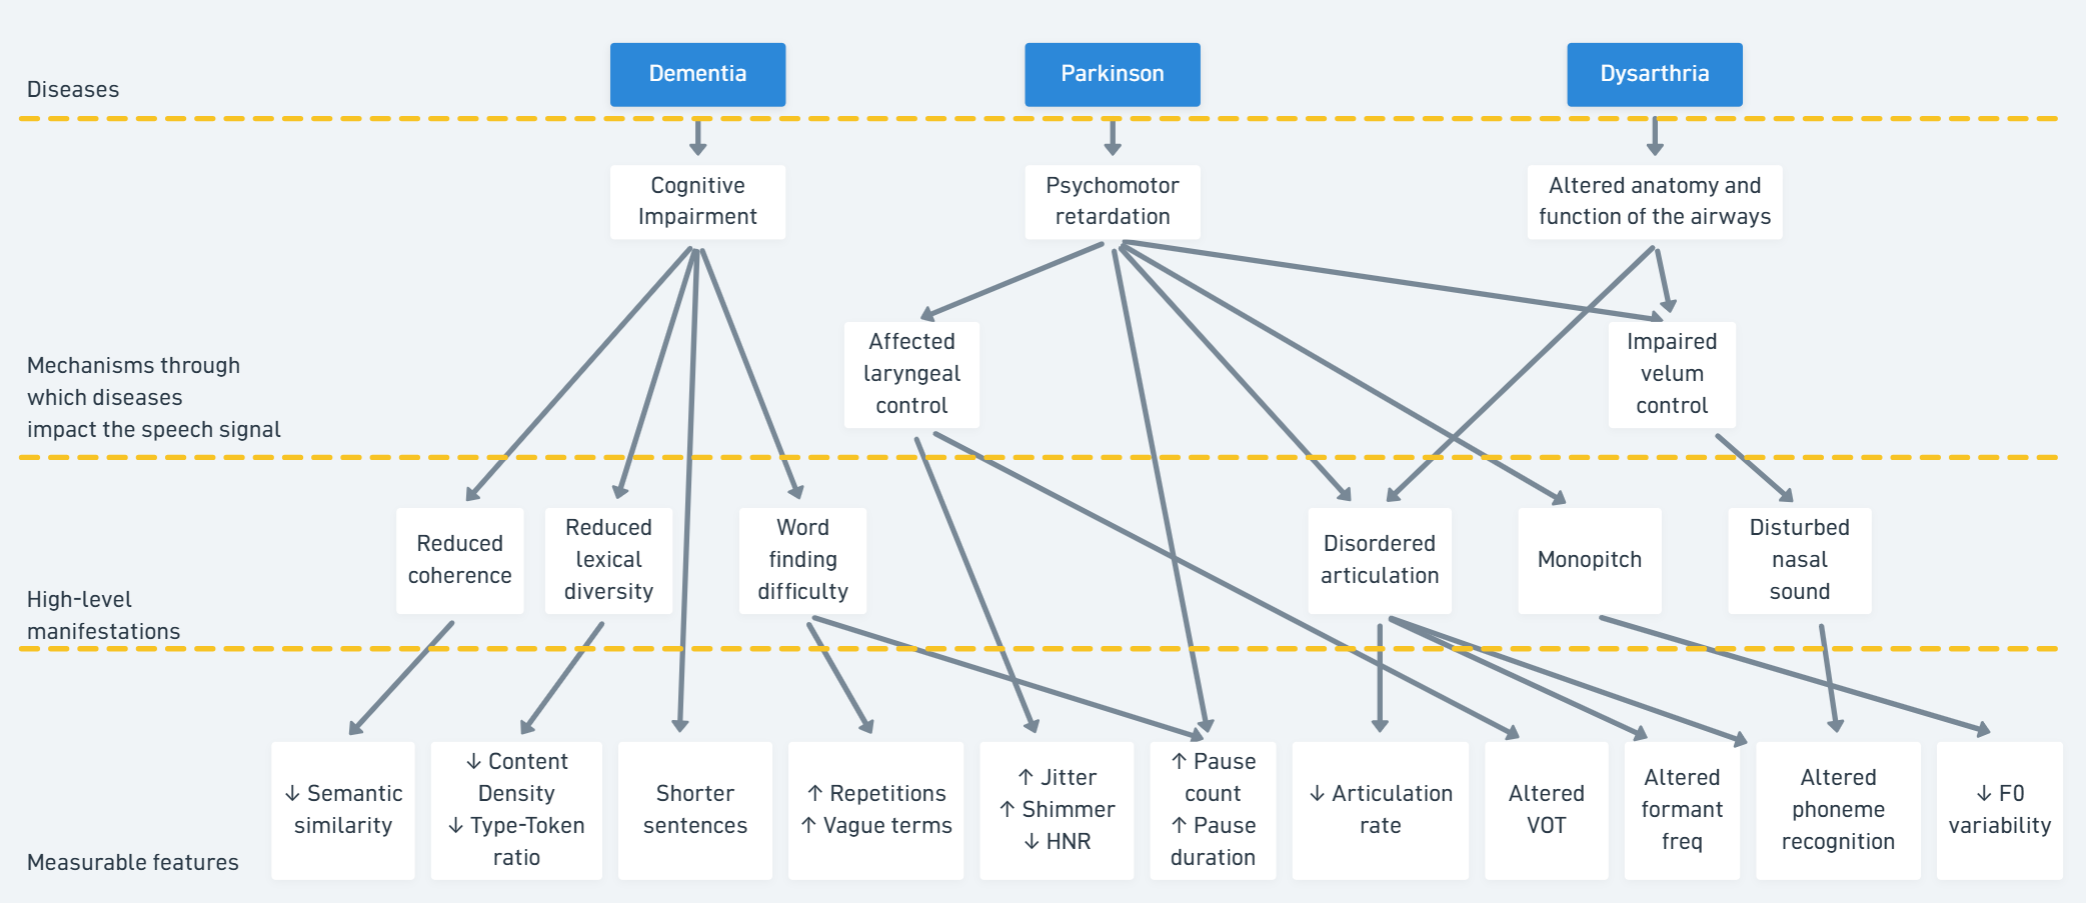
\includegraphics[width=\linewidth]{figures/symptom_to_feature.png}
\captionof{figure}{Measurable features from symptoms of three diseases\cite{10767227,xu2023dysarthria}}
\end{center}
\vspace{1cm}
%------------------------------------------------

%----------------------------------------------------------------------------------------
%	Post-Hoc examples
%----------------------------------------------------------------------------------------
\section{Post-Hoc Feature Attribution}
\boxtitle{Post-Hoc Feature Attribution}
\vspace{1cm}
\subsection*{CNN + SHAP}
\boxsubtitle{CNN + SHAP}
\begin{center}
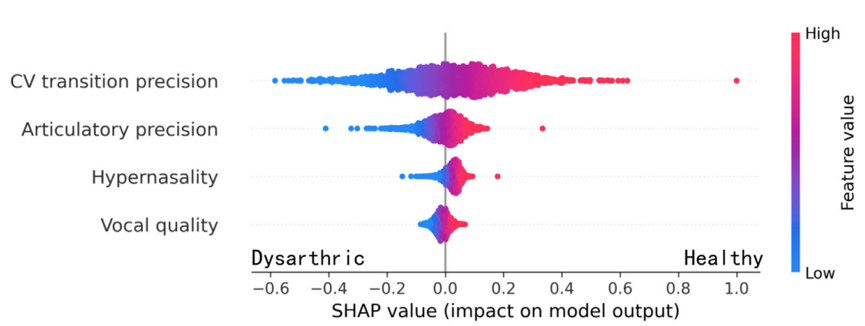
\includegraphics[width=\linewidth]{figures/Dysarthria+SHAP.png}
\captionof{figure}{Use SHAP values to illustrate how each feature affect model decision\cite{xu2023dysarthria}}
\end{center}
\vspace{1cm}
\subsection*{BERT + LIME}
\boxsubtitle{BERT + LIME}
\begin{center}
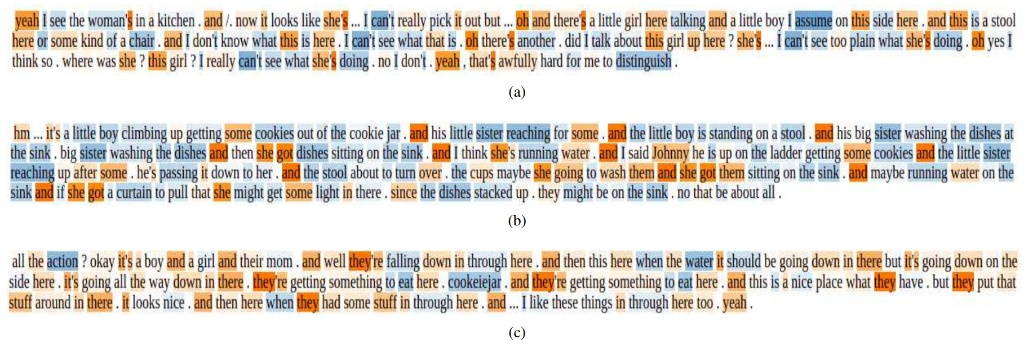
\includegraphics[width=\linewidth]{figures/BERT+LIME02.jpg}
\captionof{figure}{Label: Dementia, Prediction: Dementia\cite{Ilias_2022}}
\end{center}
\vspace{1cm}

%----------------------------------------------------------------------------------------
%	Limitations
%----------------------------------------------------------------------------------------
\section{Limitations of Post-Hoc Methods}
\boxtitle{Limitations of Post-Hoc Methods}
\vspace{1cm}
\begin{center}
\begin{minipage}{\linewidth} 
    \large 
    \renewcommand{\arraystretch}{1.5} 
    \begin{tabularx}{\linewidth}{|>{\raggedright\arraybackslash}p{0.3\linewidth} |>{\raggedright\arraybackslash}X|} 
        \hline
        \textbf{Category} & \textbf{Description}\\ \hline
        \textbf{Computational Complexity} & High cost of SHAP with a large neural network\\ \hline
        \textbf{Reliability} & Inconsistency across similar instances by LIME\\ \hline
        \textbf{Lack of Evaluation Metrics} & Difficulties in comparison across studies\\ \hline
        \textbf{Feature Dependency} & Cannot decode uninterpretable input\\ \hline
    \end{tabularx}  
    \captionof{table}{Drawbacks of post-hoc interpretation\cite{11371361}}
\end{minipage}
\end{center}
\vspace{1cm}

%----------------------------------------------------------------------------------------
%	Concept-based architectures
%----------------------------------------------------------------------------------------
\section{Beyond Black-Box: Predictions Through Clinical Concepts}
\boxtitle{Beyond Black-Box: Predictions Through Clinical Concepts}
\vspace{1cm}

%----------------------------------------------------------------------------------------
\subsection*{Concept Bottleneck Models (CBM)}
\boxsubtitle{Concept Bottleneck Models (CBM)}
\vspace{0.5cm}

The model predicts named clinical symptoms before classifying.
An LLM (Gemini-pro) annotates training data from unstructured
medical notes --- at test time, only the audio model runs.

\begin{center}
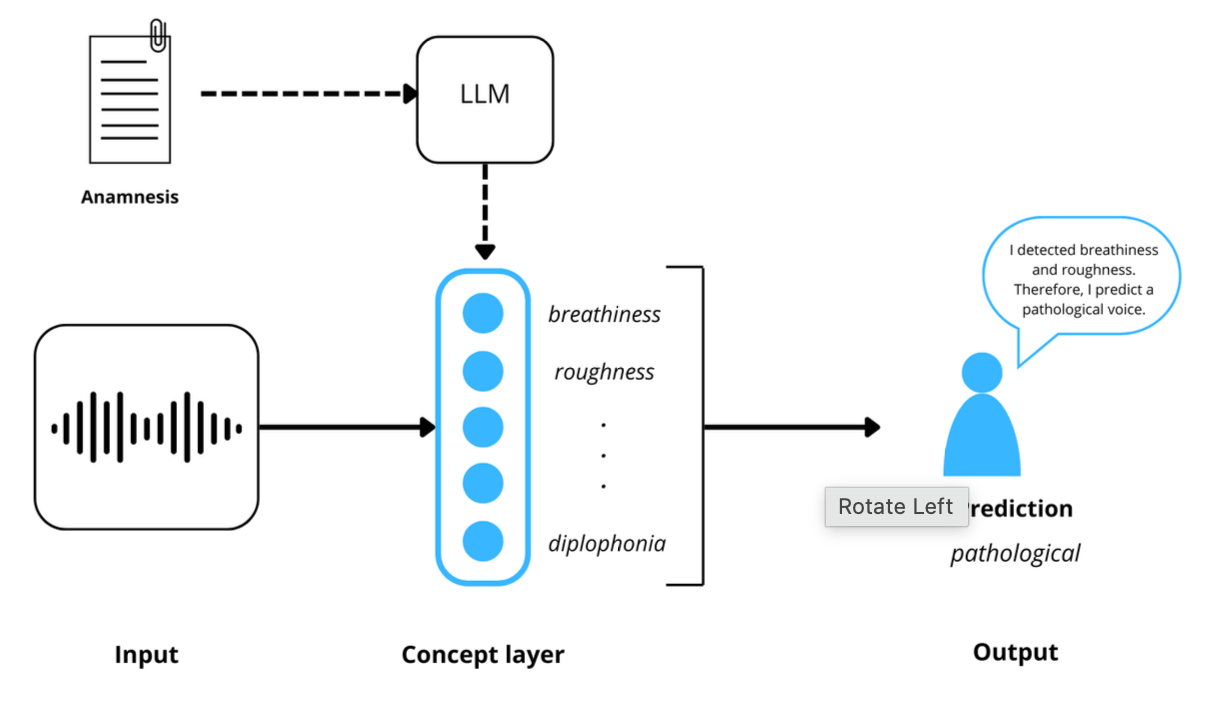
\includegraphics[width=\linewidth]{figures/cbm_framework.png}
\captionof{figure}{Audio mapped through a clinical concept layer
before prediction. LLM used at training only
(dashed)\cite{ghia2025conceptbasedapproachvoicedisorder}.}
\end{center}
\vspace{0.5cm}

\begin{center}
\renewcommand{\arraystretch}{1.5}
\begin{tabularx}{\linewidth}{|>{\raggedright\arraybackslash}p{0.25\linewidth}
                              |>{\raggedright\arraybackslash}X
                              |>{\raggedright\arraybackslash}X|}
\hline
\textbf{Dimension} & \textbf{Ghia et al. \cite{ghia2025conceptbasedapproachvoicedisorder}} & \textbf{Leschly et al. \cite{1e0730b6d8ef423d89d5860c23834a1b}} \\ \hline
\textbf{Role of Text}
  & \textbf{Training phase only:} LLM extracts clean target labels from unstructured notes offline\cite{ghia2025conceptbasedapproachvoicedisorder}.
  & \textbf{Live test input:} Transcribed words are converted to BERT embeddings during execution\cite{1e0730b6d8ef423d89d5860c23834a1b}. \\ \hline
\textbf{Inference Input}
  & \textbf{Audio only:} Discards text at test time; relies strictly on HuBERT speech encoder\cite{ghia2025conceptbasedapproachvoicedisorder}.
  & \textbf{Multimodal fusion:} Requires both raw speech (wav2vec 2.0) and text (BERT) streams\cite{1e0730b6d8ef423d89d5860c23834a1b}. \\ \hline
\textbf{Concept Targets}
  & \textbf{Vocal acoustics:} Evaluates physical sound quality (e.g., breathiness, roughness, strain)\cite{ghia2025conceptbasedapproachvoicedisorder}.
  & \textbf{Patient symptoms:} Tracks holistic functional complaints (e.g., pain, gait decline, tremors)\cite{1e0730b6d8ef423d89d5860c23834a1b}. \\ \hline
\end{tabularx}
\captionof{table}{Text serves fundamentally opposite roles across concept-based diagnostic frameworks.}
\end{center}
\vspace{1cm}

%----------------------------------------------------------------------------------------
\subsection*{From Binary Nodes to Embeddings: CEM}
\boxsubtitle{From Binary Nodes to Embeddings: CEM}
\vspace{0.5cm}

CBM assigns one binary node per concept. CEM replaces it with
an active/inactive embedding pair --- richer and equally
interpretable.

\begin{center}
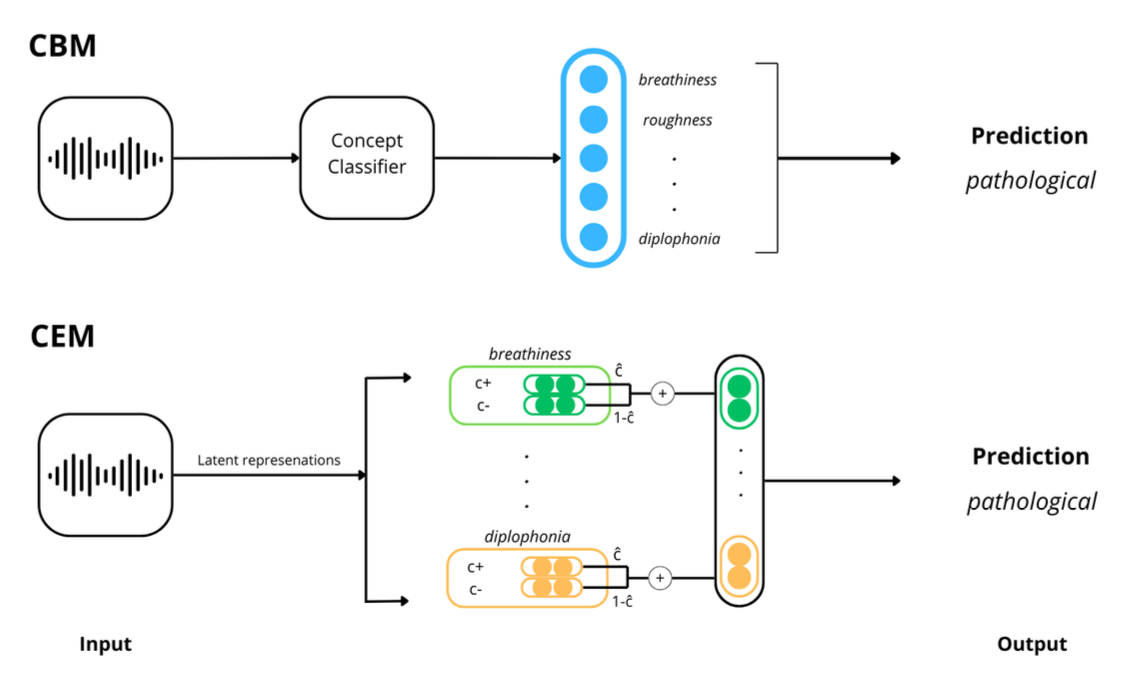
\includegraphics[width=\linewidth]{figures/cbm_cem_architecture.png}
\captionof{figure}{CBM vs.\ CEM: binary nodes vs.\
embedding pairs per vocal concept\cite{ghia2025conceptbasedapproachvoicedisorder}.}
\end{center}
\vspace{1cm}

%----------------------------------------------------------------------------------------
\subsection*{Literature-Grounded Explanations (RAG)}
\boxsubtitle{Literature-Grounded Explanations (RAG)}
\vspace{0.5cm}

Predicted concepts retrieve peer-reviewed evidence and generate
a clinician-readable report --- no post-hoc step needed.

\begin{center}
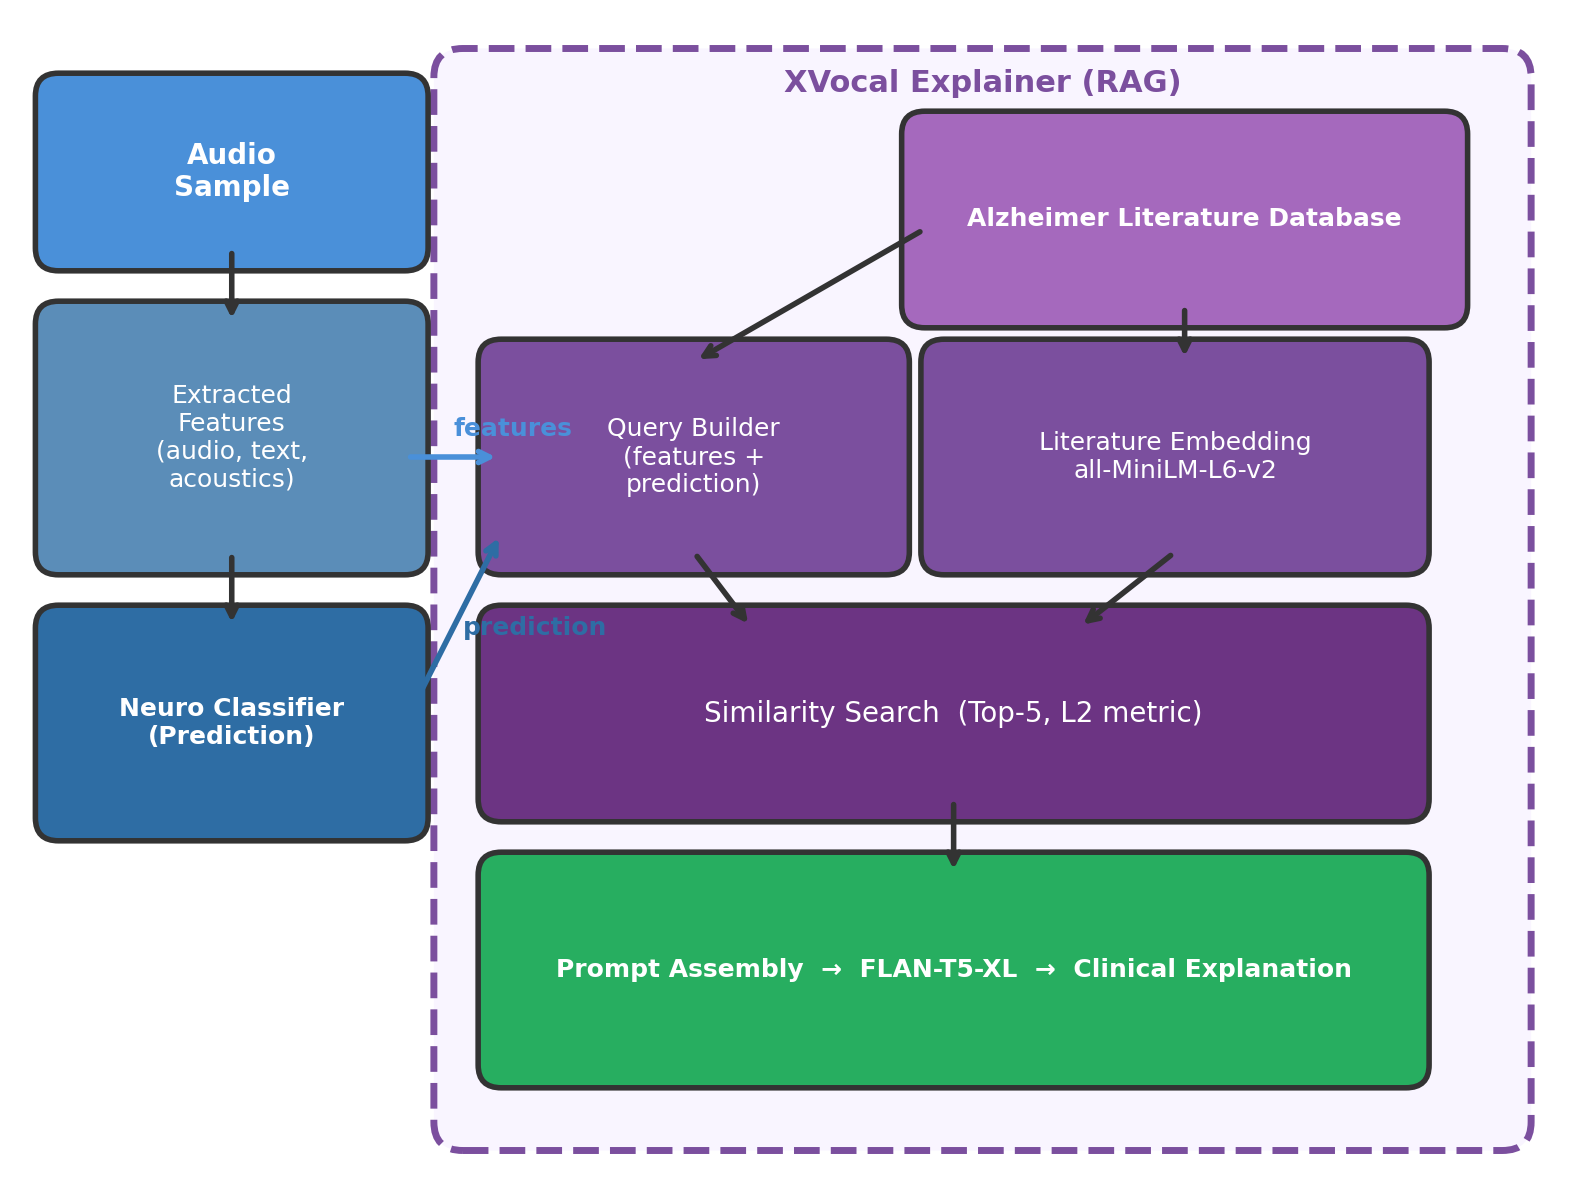
\includegraphics[width=\linewidth]{figures/neuroxvocal.png}
\captionof{figure}{NeuroXVocal: concepts drive RAG retrieval
from medical literature, producing evidence-grounded
reports\cite{Ntampakis_2025}.}
\end{center}
\vspace{1cm}

%----------------------------------------------------------------------------------------
\subsection*{Results}
\boxsubtitle{Results}
\vspace{0.5cm}

\begin{center}
\renewcommand{\arraystretch}{1.5}
\begin{tabularx}{\linewidth}{|>{\raggedright\arraybackslash}p{0.24\linewidth}
                              |>{\raggedright\arraybackslash}X
                              |>{\centering\arraybackslash}p{0.20\linewidth}|}
\hline
\textbf{Task} & \textbf{Model} & \textbf{Score} \\ \hline
\multirow{2}{*}{Voice disorder}
  & HuBERT black-box    & 0.909 F1 \\
  & CEM                 & 0.860 F1 \\ \hline
\multirow{2}{*}{Dysarthria}
  & Black-box CNN       & 82.5\% Acc \\
  & + concept layer     & \textbf{83.9\%} Acc \\ \hline
\multirow{2}{*}{MCI}
  & Baseline            & 0.58 AUC \\
  & + concept layer     & \textbf{0.62 AUC} \\ \hline
Alzheimer's
  & NeuroXVocal         & \textbf{0.958 F1} \\ \hline
\end{tabularx}
\captionof{table}{Concept-based models match or exceed
black-box baselines across all four disorders.}
\end{center}

\vspace{0.5cm}
\colorbox{yellow!10}{%
  \parbox{\dimexpr\linewidth-2\fboxsep}{%
    \LARGE
    \textbf{\color{Black}Key Finding:} Concept-based models
    predict \textit{through} clinical symptoms ---
    accurate, transparent, no post-hoc approximation.
  }%
}
\vspace{1cm}


%----------------------------------------------------------------------------------------
%	REFERENCES
%----------------------------------------------------------------------------------------

\boxtitle{References}
\vspace{0.5cm}

\begin{center}

\includegraphics[width=0.45\linewidth]{figures/references_qr.png}\\[0.5cm]
\Large Scan for the full reference list\\
\url{https://github.com/gloriagalasso/What-Do-Clinical-Speech-Models-Actually-Learn-}
\end{center}

%----------------------------------------------------------------------------------------

\end{multicols}

\end{document}


%% --- END OF FILE